\documentclass[12pt, oneside]{article}   	
\usepackage{geometry}                		% See geometry.pdf to learn the layout options. There are lots.
\geometry{letterpaper}                   		% ... or a4paper or a5paper or ... 
\usepackage{graphicx}				% Use pdf, png, jpg, or eps§ with pdflatex; use eps in DVI mode
\usepackage{amssymb}
\usepackage[spanish]{babel}
\usepackage{csquotes}
\usepackage{url}
\usepackage{amsmath}
\usepackage{float} %para las figuras

\newcommand{\speaker}[1]{\textbf{#1:}}

\title{Un puntito más que tú \\ \vspace{0.5em}
\large Un análisis dimensional de las funciones del cariño}
\author{Jorge A. Saldaña}
\date{\today}							% Activate to display a given date or no date

\begin{document}
\maketitle

\section{Introducción}
\label{sec:intro}
Cuando dos personas, llamémosles persona \textbf{a} y perosona \textbf{b} que experimentan un amor mutuo 
(y ambas son competitivas) expresan su cariño, puede ocurrir el evento descrito en la figura \ref{fig:conversacion1} 

\begin{figure}[h]
\centering % centra el bloque completo
\begin{minipage}{0.7\linewidth} % ancho del bloque (ajústalo)
\raggedright % dentro del bloque, alinea a la izquierda
\label{fig:conversacion1}

\speaker{a} Te amo.

\speaker{b} Yo te amo más.

\speaker{a} Yo un puntito más que tú.

\speaker{b} Yo una línea más que tú.

\speaker{a} Yo un sólido revolucionado más que tú.

\end{minipage}
\caption{Conversación normal entre dos personas que se aman}
\end{figure}

Iniciando así una reacción en cadena en la que cada persona busca ser la que ama más a su pareja.

Si ponemos atención, pareciera que cada persona va aumentando su cariño en una dimensión espacial, lo que inspira la 
pregunta:
\textbf{¿Qué significa} cada una de estas dimensiones espaciales?, ¿qué propiedades tienen y qué medidas podemos 
sacar de ellas?

Este escenario recuerda también al descrito en un fascinante fragmento de la novela \textit{El problema de los tres 
cuerpos}, del autor chino Liu Cixin, en el que\footnote{Sin afán de hacer más \textit{spoiler}} los habitantes del 
planeta Trisolaris ``desdoblan'' un protón en las diferentes dimensiones, resultando tener en estas un tamaño 
infinitamente más grande en el que pudieron grabar circuitos y guardar programas, para finalmente volver a ``doblar'' dicho protón a su dimensión original y tener así una computadora súper potente de tamaño subatómico\cite{liu2016trescuerpos}.

Con este nuevo panorama, exploremos entonces las dimensiones en las que (al menos en la ciencia ficción) podemos 
expresar el cariño y desdoblar protones.

\section{El punto}
\label{sec:punto}
En geometría, el punto es un concepto fundamental que representa una ubicación en el espacio~\cite{eswiki:punto}. 
Solemos pensar en los puntos y representarlos gráficamente como un círculo pequeño, como se ilustra en la figura~\ref{fig:grafPunto} pero en realidad un círculo por más pequeño que sea tiene área y circunferencia, lo que sólo puede darse a partir de la segunda dimensión, como veremos más adelante.

\begin{figure}[h]
\centering
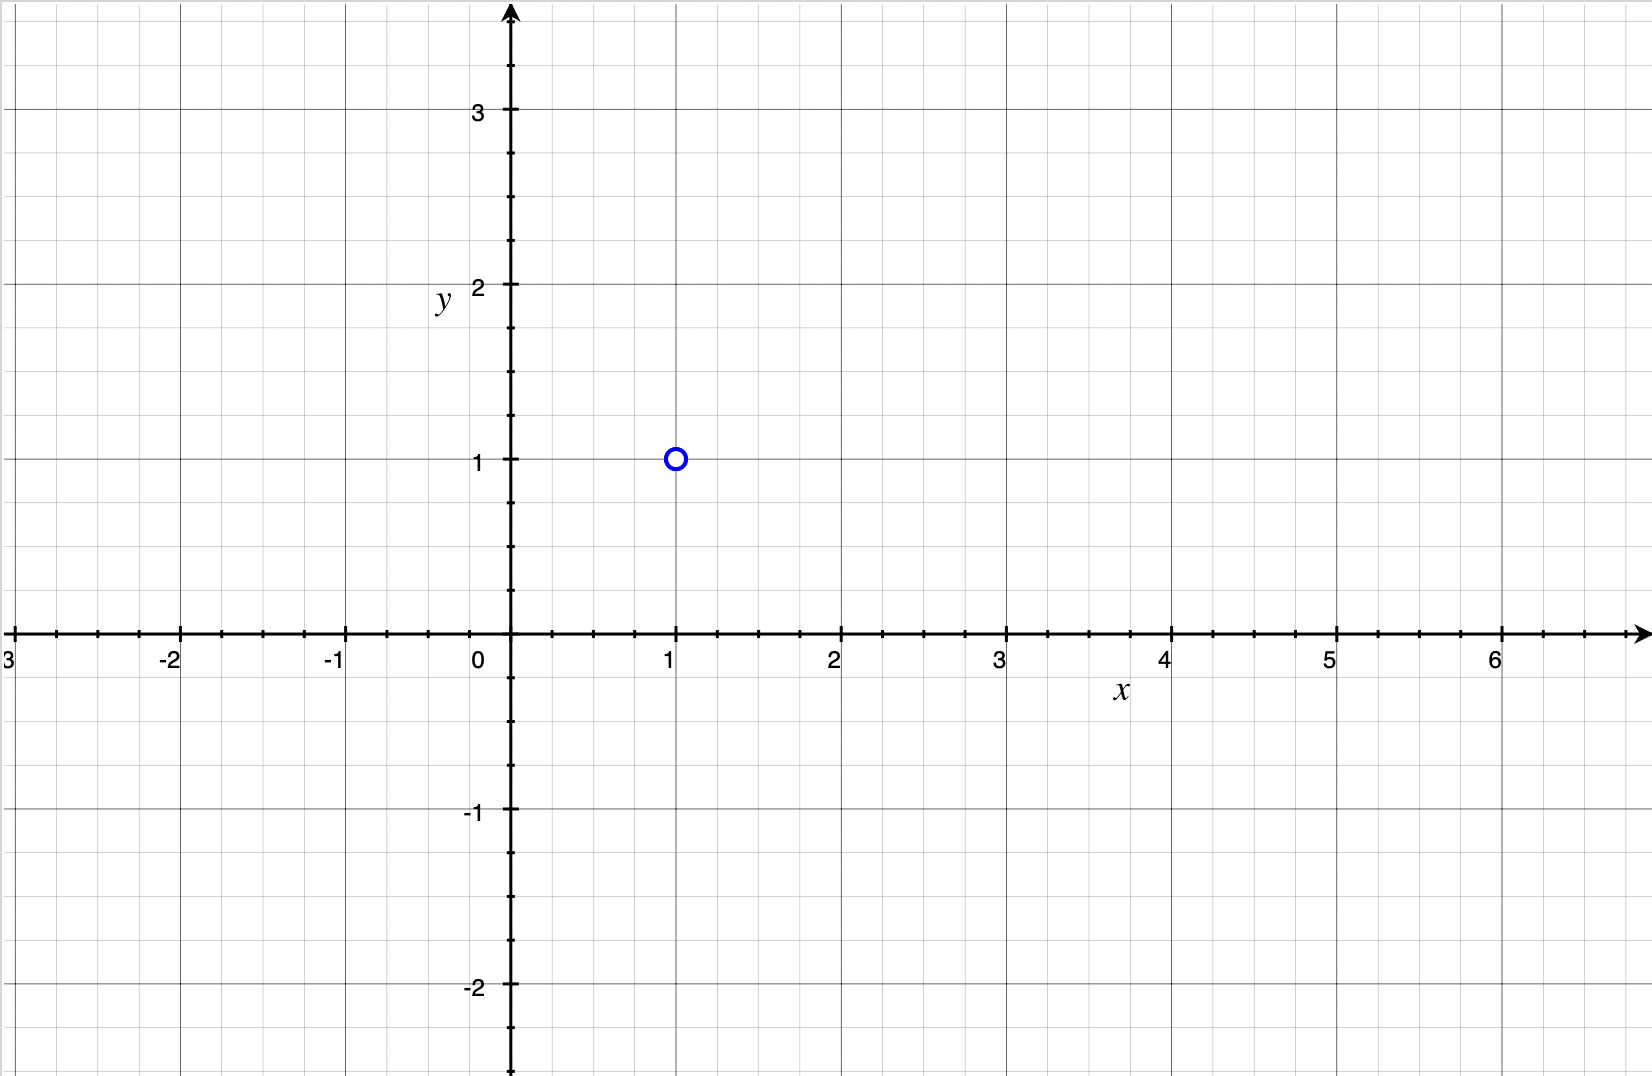
\includegraphics[width=0.6\textwidth]{grafPunto.png}
\caption{Representación gráfica de un punto en las coordenadas (1,1)}
\label{fig:grafPunto}
\end{figure}

El punto es la unidad más simple, una figura geométrica \textbf{sin} dimensión: no tiene longitud, área, volumen, ni otro ángulo dimensional; es decir, existe en cero dimensiones~\cite{book:Geometry4Teach}.

Podemos entonces interpretar que querer un \textit{puntito más} es una forma sutil de querer de una forma infinitesimal, que siempre se acerca a un valor, de forma parecida a los límites, como se ilustra en la ecuación~\ref{eq:puntito}.

\begin{equation}
\label{eq:puntito}
\lim_{x \to 1^+} x = 1^+
\end{equation}

Aquí, $1^+$ indica “uno por arriba”, es decir, apenas mayor que uno.

\section{La línea}
\label{sec:linea}
En geometría, la línea o \textbf{recta} puede describirse como una sucesión contínua de puntos extendidos en una sola dimensión.

Como se mencionó brevemente al inicio de la sección~\ref{sec:punto}, la línea es también un concepto fundamental de la geometría, esto quiere decir que sólo puede describirse a partir de la descripción de otros elementos similares, como en este caso es el punto~\cite{eswiki:recta}.

La recta existe en una dimensión, se extiende en una dirección y tiene una cierta longitud, la cuál puede ser infinita.

Algunos ejemplos de rectas se muestran en la figura~\ref{fig:grafRectas}.
\begin{figure}[h]
\centering
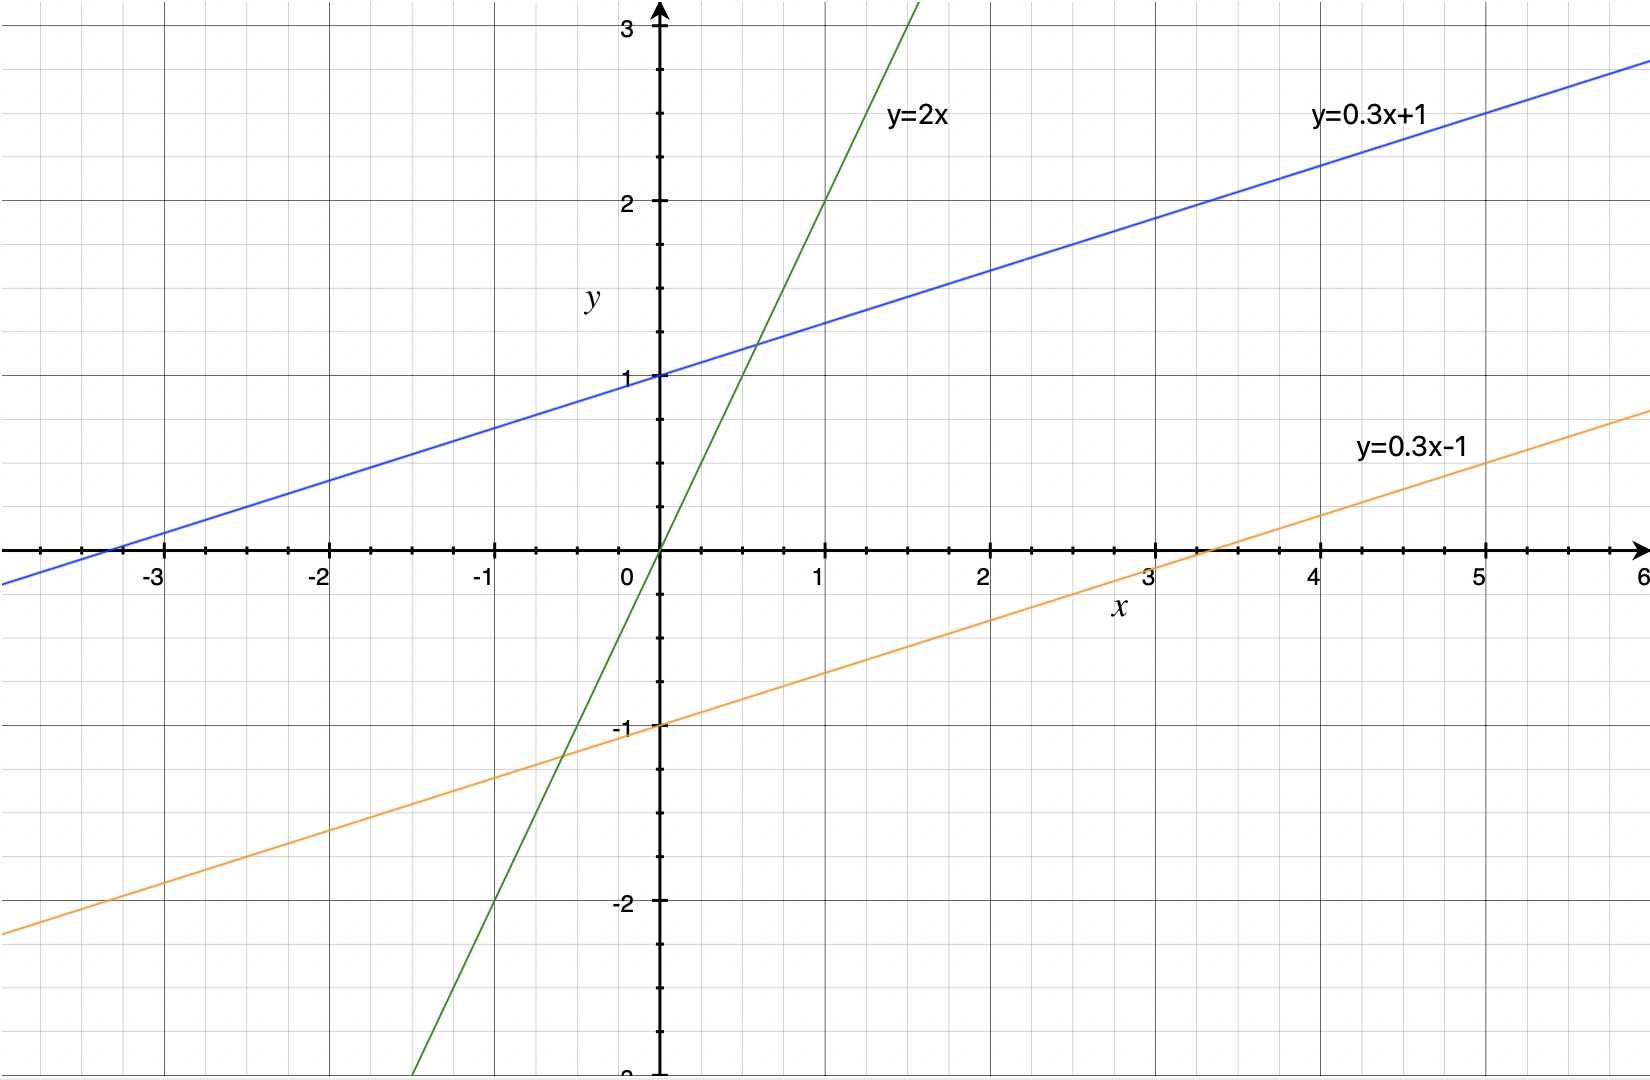
\includegraphics[width=0.6\textwidth]{grafRectas.png}
\caption{Ejemplos de rectas en un plano.}
\label{fig:grafRectas}
\end{figure}

Interpretaremos entonces que querer \textit{una línea más} es querer una cantidad infinita de puntos en la misma dirección.

\section{El plano}
\label{sec:plano}
Habiendo definido elementos fundamentales de la geometría como lo son el punto y la línea, resulta ahora necesario introducir el concepto de plano.

Formalmente, el plano cartesiano es un sistema de referencia que nos permite representar un espacio en dos dimensiones
mediante dos líneas perpendiculares llamadas ejes, siendo comunmente la horizontal el eje $x$ o de las \textit{absisas} y la vertical el eje $y$ o de las \textit{ordenadas}; las cuales se intersectan en el origen~\cite{eswiki:planoCartesiano}.

El plano permite a su vez utilizar un sistema de coordenadas para representar cualquier punto $P = (x, y)$, siendo el origen el punto $(0,0)$.

Utilizando el sistema de coordenadas del plano cartesiano, podemos representar elementos geométricos como el punto y la recta por medio de ecuaciones.

\subsection{Ecuación de la recta}
Dada una recta mediante un punto $P=(x_1, y_1)$ y una pendiente $m$ se puede obtener la ecuación de la recta conocida como punto pendiente:

\begin{equation}
\label{eq:puntoPendiente}
y-y_1 = m(x-x_1)
\end{equation}

Si se conoce la pendiente $m$, y el punto donde la recta corta al eje de ordenadas es $(0,b)$ podemos deducir partiendo de la ecuación punto pendiente una forma simplificada:

\begin{equation}
\begin{aligned}
y - y_1 &= m(x - x_1) \\
y - b   &= m(x - 0) \\
y - b   &= mx \\
y       &= mx + b
\end{aligned}
\end{equation}

Existen otras formas de representar rectas mediante ecuaciones que utilizan el sistema de coordenadas cartesianas pero quedan fuera del interés de este texto.

\section{La función matemática}
En análisis matemático, el concepto general de función, se refiere a una regla que asigna a cada elemento de un primer conjunto un único elemento de un segundo conjunto~\cite{eswiki:funcionMat}.

Las funciones matemáticas nos son reelevantes a nuestro análisis del cariño porque permiten generar un conjunto infinito de pares entrada-salida que pueden respectivamente tabularse como puntos en un plano.
Observemos algunos ejemplos de esto en la figura~\ref{fig:grafFunciones}.

\begin{figure}[h]
\centering
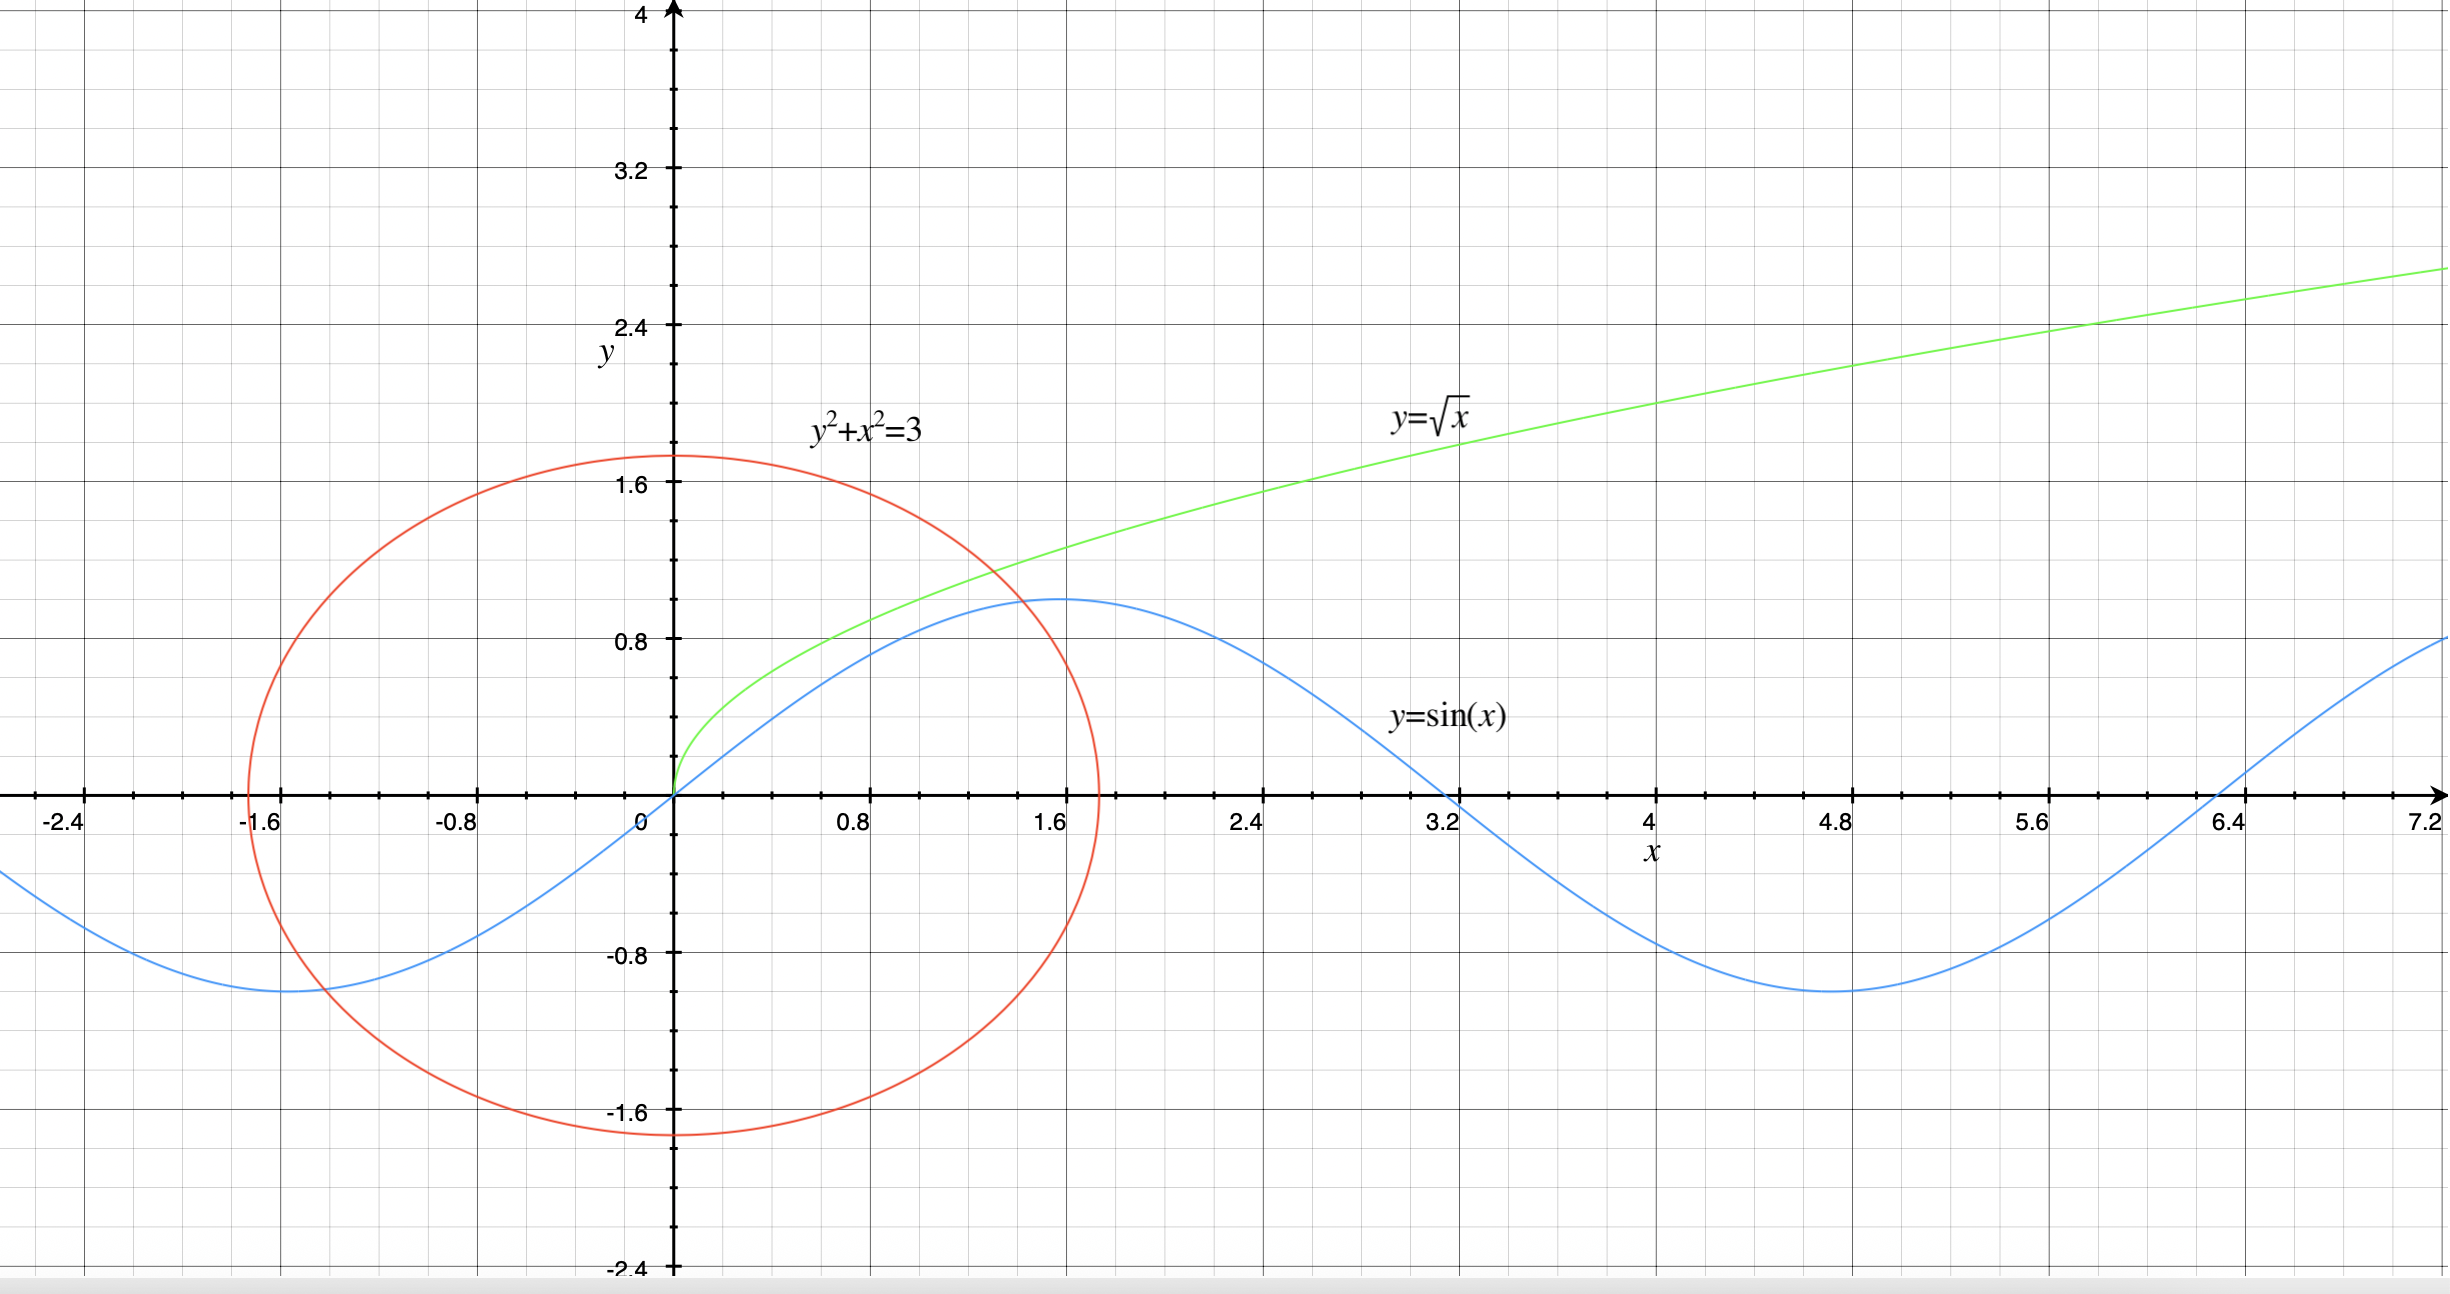
\includegraphics[width=0.6\textwidth]{grafFunciones.png}
\caption{Ejemplos de gráficas de funciones matemáticas.}
\label{fig:grafFunciones}
\end{figure}

Ahora con los conceptos de plano y función definidos, podemos continuar con nuestro análisis dimensional del cariño, 
pues podemos modelar las infinitas expresiones del amor con una equivalentemente infinita diversidad de funciones 
matemáticas: algunas suben y bajan de forma periódica, otras que van en círculos o parecen tender a la constancia hacia
 el infinito, etc.

\section{El área bajo la curva}
Una propiedad bidimensional que podemos calcular en muchas funciones matemáticas es el área bajo la curva, es decir, 
el área de la región del plano comprendida entre la gráfica de la función $f(x)$, el eje $x$, y las líneas verticales 
$x = a$ y $x = b$.\cite{eswiki:integracion} 

Este cálculo corresponde a la integral definida de la función entre esos límites, como se muestra en la 
ecuación~\ref{eq:integDefinida}:

\begin{equation}
\label{eq:integDefinida}
\int_{a}^{b} f(x)\, dx
\end{equation}

Para ilustrarlo con un ejemplo, consideremos de forma arbitraria la función \mbox{$f(x) = \sqrt{x}$} como modelo de nuestro 
cariño. El área bajo su curva, entre los valores $0$ y $8$ en el eje de las abscisas, representa entonces la magnitud 
total de ese cariño dentro de dicho intervalo.

\begin{equation}
\begin{aligned}
\int_{0}^{8} \sqrt{x}\, dx &= \int_{0}^{8} x^{1/2}\, dx = \frac{2}{3}x^{3/2}\Big|_{0}^{8} \\[0.5em]
&= \frac{2}{3}(8^{3/2} - 0^{3/2}) \\[0.5em]
&= \frac{2}{3}\sqrt{8^3} \\[0.5em]
&= \frac{32}{3}\sqrt{2} \approx 15.0849
\end{aligned}
\label{eq:integSqrt}
\end{equation}

El resultado, por supuesto, debe medirse en unidades cuadradas y el ejemplo del procedimiento~\ref{eq:integSqrt}
puede verse ilustrado en la figura~\ref{fig:grafIntDef}.

\begin{figure}[h]
\centering
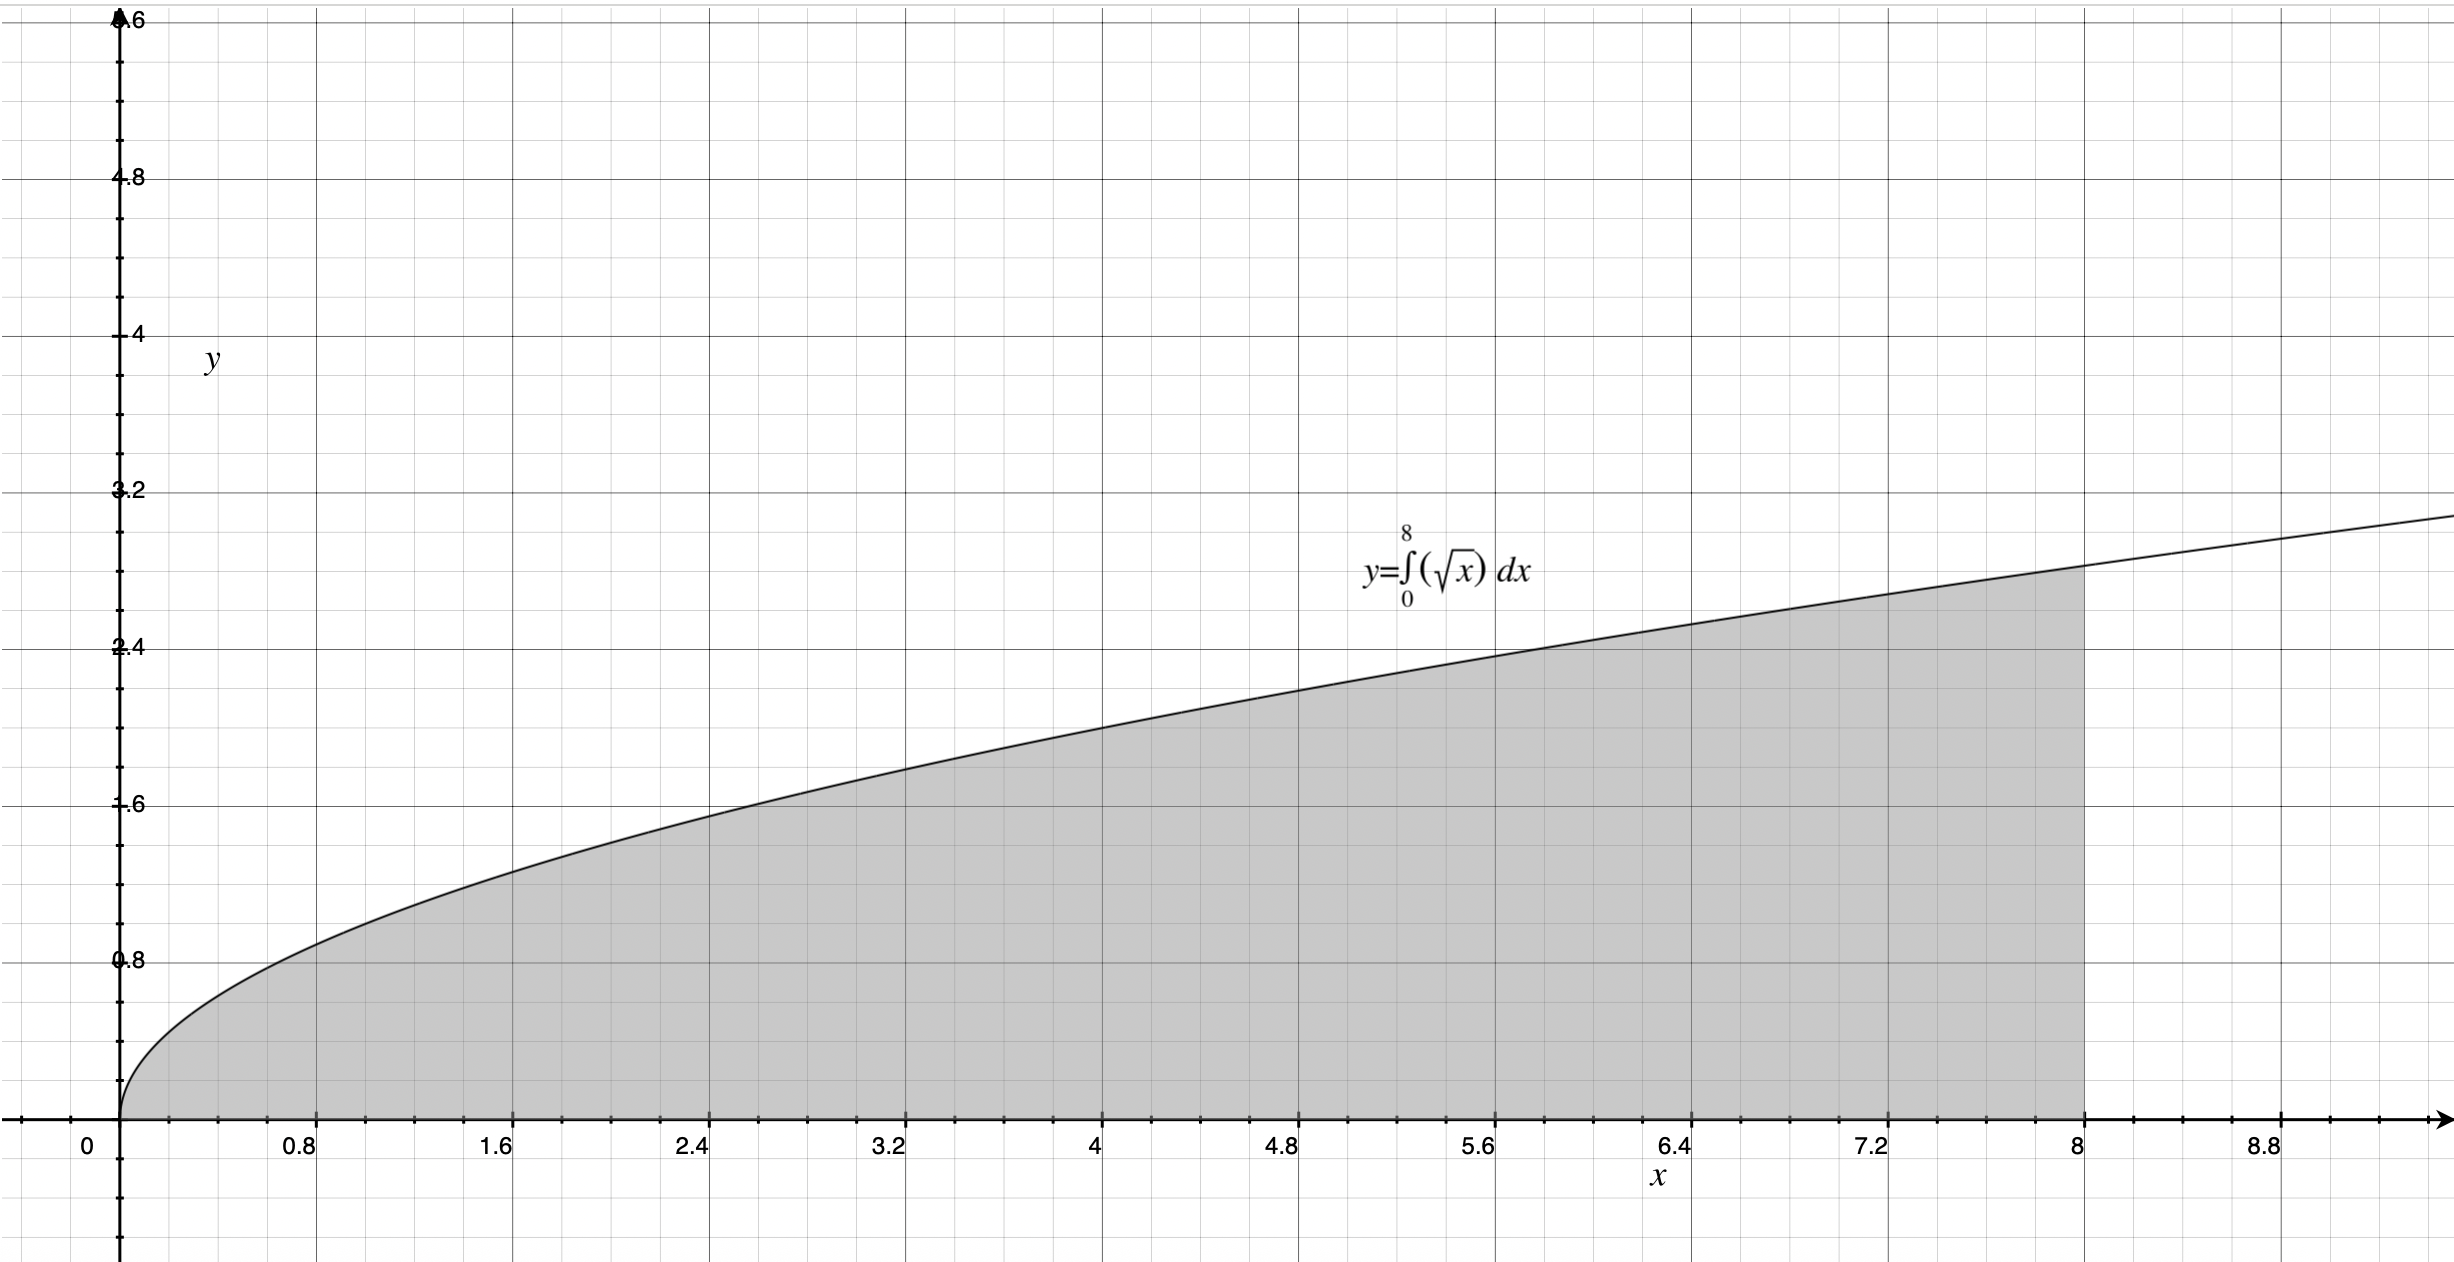
\includegraphics[width=0.8\textwidth]{grafIntDef.png}
\caption{Ejemplo del área bajo la curva utilizando la integral definida de una función matemática.}
\label{fig:grafIntDef} % <- aquí después del caption
\end{figure}

%Dale interpretación de cariño
Una posible interpretación metafórica de esta medición podría ser que, dentro de esta superficie, podrían dibujarse una infinidad de líneas, tantas que cubran el equivalente al área total de la figura delimitada entre la función y el eje de las abscisas.

\section{El sólido de revolución}
Un sólido de revolución es aquel que se obtiene al rotar una curva plana alrededor de un eje que se encuentra en el mismo plano de la curva, llamado \textit{eje de revolución}. 

Por ejemplo, si consideramos la región comprendida entre la función $y = f(x)$, el eje $x$ ($y=0$), y las líneas verticales $x=a$ y $x=b$, y hacemos girar esta región alrededor del eje $x$, se genera un sólido cuya forma es determinada por la rotación. 

El volumen de este sólido puede calcularse utilizando el \textbf{método de los discos}, que consiste en imaginar la región subdividida en rectángulos infinitesimales de base $dx$ y altura $f(x)$. Al girar cada rectángulo alrededor del eje $x$, se forma un disco con volumen $\pi [f(x)]^2 dx$. Sumando infinitamente estos discos a lo largo del intervalo $[a,b]$, obtenemos la integral:

\begin{equation}
V = \pi \int_{a}^{b} [f(x)]^2\, dx
\label{eq:volSolidoRevolucion}
\end{equation}

De esta manera, el cálculo del volumen de sólidos generados por rotación se reduce a una integral definida de la función que delimita la región~\cite{eswiki:solidoRevolucion}.

%Ahora pon el ejemplo con \sqrt{x}
Continuando el ejemplo de la sección anterior, donde el área bajo la curva representaba la extensión de nuestro cariño, ahora imaginemos cómo sería si ese cariño girara completamente sobre sí mismo; con la función \mbox{$f(x) = \sqrt{x}$} para $0 \leq x \leq 8$, 
resolvemos:

\begin{equation}
\begin{aligned}
V &= \pi \int_{0}^{8} [\sqrt{x}]^2\, dx \\[0.5em]
&= \pi \int_{0}^{8} x\, dx \\[0.5em]
&= \pi \cdot \frac{x^2}{2} \Big|_{0}^{8} \\[0.5em]
&= \frac{\pi}{2} \cdot (8^2 - 0^2) = 32\pi \approx 100.531
\end{aligned}
\label{eq:ejSolRev}
\end{equation}

El resultado debe interpretarse en unidades cúbicas y el ejemplo del procedimiento~\ref{eq:ejSolRev}
puede verse ilustrado en la figura~\ref{fig:grafSolRev}, con la aclaración de que en dicha figura se muestra únicamente la superficie del sólido generado por la rotación, es decir, su contorno, no su volumen lleno.

\begin{figure}[H]
\centering
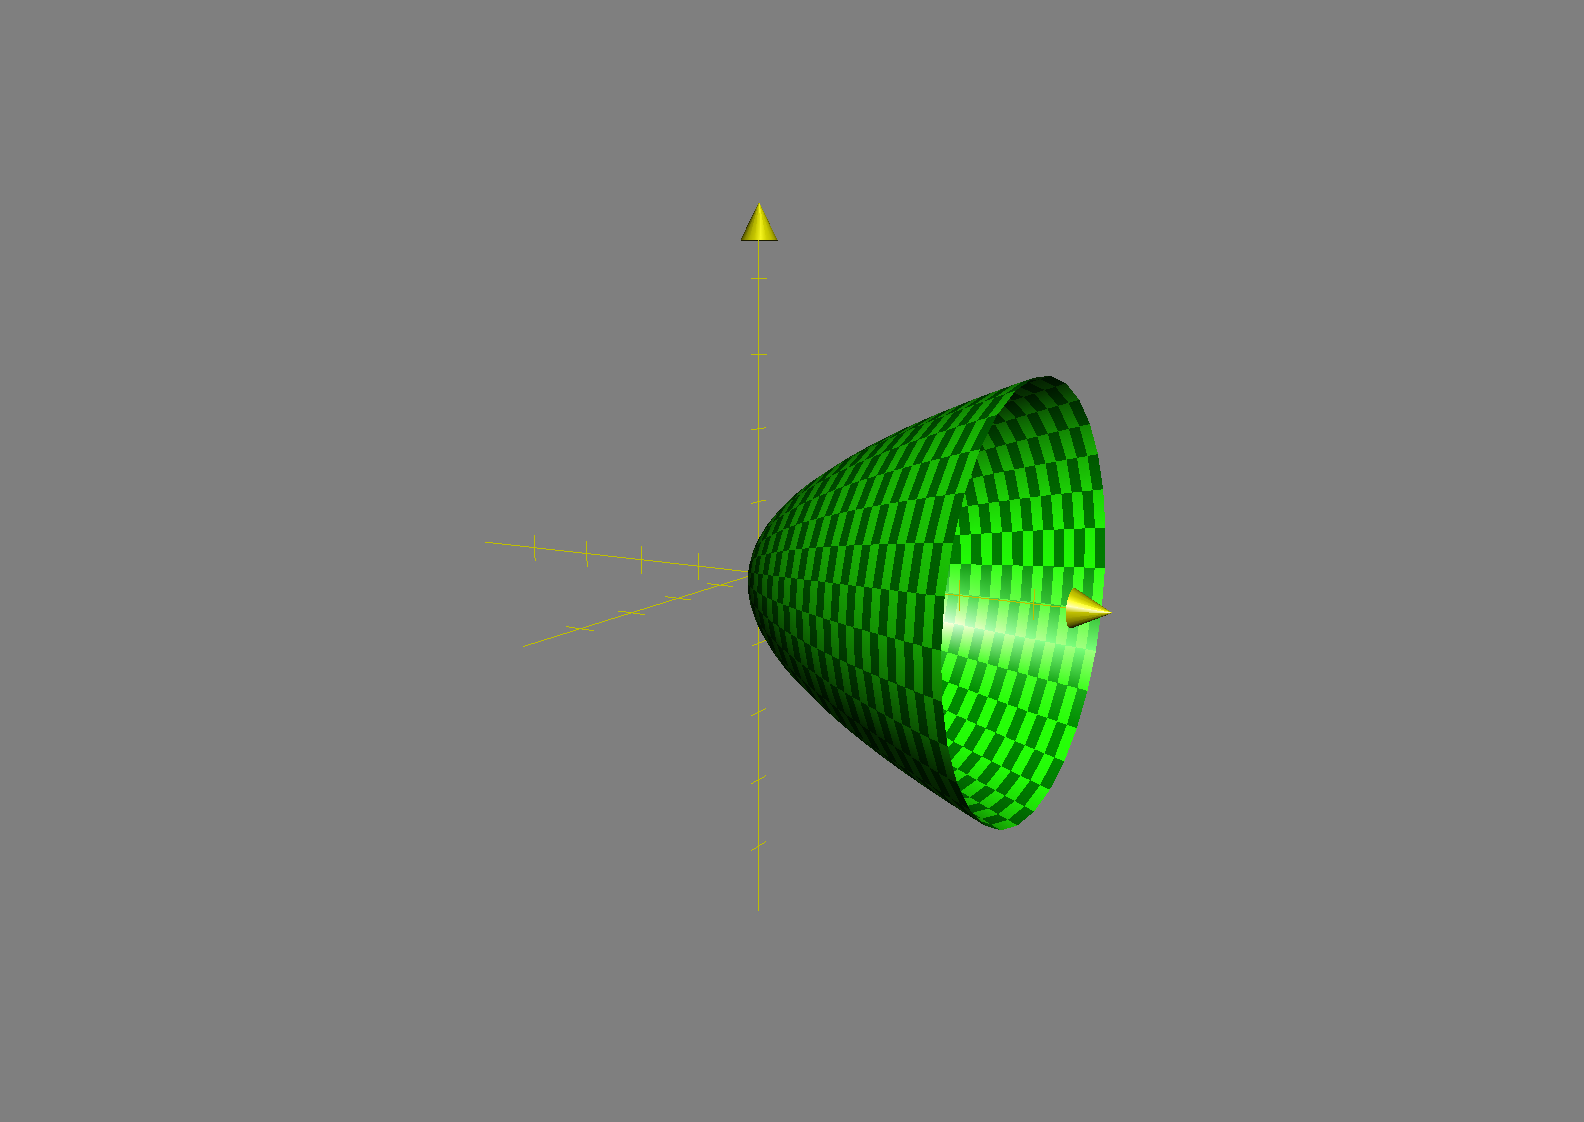
\includegraphics[width=0.7\textwidth]{grafSolRev.png}
\caption{Sólido de revolución de la función $f(x) = \sqrt{x}$}
\label{fig:grafSolRev} % <- aquí después del caption
\end{figure}

%Dale la interpretación del cariño
Finalmente, la interpretación metafórica que podemos darle a este sólido revolucionado de cariño, frente al área bajo la curva, es que el método de los discos nos invita a imaginar una cantidad infinita de superficies de nuestra función, apiladas una sobre otra, formando una presencia más densa, más profunda: un cariño que ya no sólo se extiende, sino que adquiere volumen.

\section{Las Hiperdimensiones}
Se conoce como espacio hiperdimensional o \textit{hiperdimensiones} al conjunto de dimensiones geométricas y físicas que comienzan a partir de la cuarta dimensión en adelante~\cite{eswiki:hiperespacio}.

Aunque imaginar estas dimensiones es menos intuitivo, las matemáticas nos permiten trabajar con ellas y describir sus propiedades.

Sin embargo, el presente análisis del cariño dimensional se limitará a la tercera dimensión, pues es aquella que experimentamos en la cotidianidad, más se deja en claro que las dimensiones superiores existen y que los conceptos que las describen pueden también aplicarse, al menos simbólicamente, a nuestra teoría del cariño.

Quizá las hiperdimensiones del cariño existan también fuera de la geometría: en los espacios invisibles y complejos donde sentimos más de lo que podemos entender y tocar.

\newpage
\bibliographystyle{unsrt} % estilo de cita (puedes cambiarlo: alpha, apalike, ieee, etc.)
\bibliography{unPuntitoMas}

\end{document}
